\documentclass[handout]{beamer}  

%Smaller gap at between top and bottom of block when there are displayed equations
\addtobeamertemplate{block begin}{\setlength\abovedisplayskip{0pt}}
{\setlength{\belowdisplayskip}{0pt}}

\usepackage{lmodern}
\usepackage{setspace}
\linespread{1.2}
\usepackage{amssymb, amsmath, amsthm} 
\usepackage{rotating}
\usepackage{multirow}
\usepackage{graphicx}
\usepackage{synttree}
\usepackage{verbatim}
\usepackage{fancybox}
\usepackage{color}
\usepackage{tikz}
\usetikzlibrary{shapes,backgrounds}
\usepackage{hyperref}
\usetikzlibrary{trees}
\newcommand{\p}{\mathbb{P}}
\newcommand{\expect}{\mathbb{E}}


%\setbeamertemplate{blocks}[rounded][shadow=true] 
%gets rid of bottom navigation bars
\setbeamertemplate{footline}{
   \begin{beamercolorbox}[ht=4ex,leftskip=0.3cm,rightskip=0.3cm]{author in head/foot}
%    \usebeamercolor{UniBlue}
    \vspace{0.1cm}
    %\insertshorttitle \ - \insertdate 
    \hfill \insertframenumber / \inserttotalframenumber
   \end{beamercolorbox}
   \vspace*{0.1cm}
} 


%gets rid of navigation symbols
\setbeamertemplate{navigation symbols}{}


%Include or exclude the notes?
%\setbeameroption{show notes}
\setbeameroption{hide notes}

\title[Econ 722]{Dynamic Factor Models} 
\author[F. DiTraglia]{Francis J.\ DiTraglia}
\institute{University of Pennsylvania}
\date{Econ 722}


\begin{document} 
%%%%%%%%%%%%%%%%%%%%%%%%%%%%%%%%%%%%%%%%



\begin{frame}[plain]
	\titlepage 
	

\end{frame} 


%%%%%%%%%%%%%%%%%%%%%%%%%%%%%%%%%%%%%%%%
\begin{frame}
\frametitle{Survey Articles on Dynamic Factor Models}

\begin{block}
	{Stock \& Watson (2010)}
	Best general overview of dynamic factor models and applications.
\end{block}

\begin{block}
	{Bai \& Ng (2008)}
Comprehensive review of large-sample results for high-dimensional factor models estimated via PCA.
\end{block}

\begin{block}
	{Stock \& Watson (2006)}
	Handbook chapter on forecasting with many predictors. One section is devoted to dynamic factor models.
\end{block}

\begin{block}
	{Breitung \& Eickmeyer (2006)}
	Brief overview with an application to Euro-area business cycles. 
\end{block}

\end{frame}
%%%%%%%%%%%%%%%%%%%%%%%%%%%%%%%%%%%%%%%%
\begin{frame}
	\frametitle{The Basic Idea}
	We're interested in settings with a large number of time series $N$ and a comparable number of time periods $T$. 
\end{frame}
%%%%%%%%%%%%%%%%%%%%%%%%%%%%%%%%%%%%%%%%
\begin{frame}[c]\frametitle{Example: Stock and Watson Dataset}
    

	\begin{figure}
		\centering
		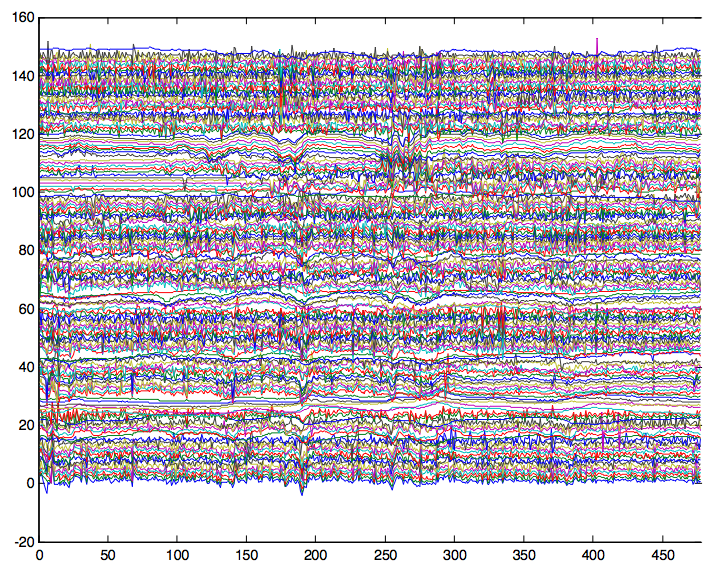
\includegraphics[scale = 0.3]{../img/stock_watson_dataset}
	\end{figure}
Monthly Macroeconomic Indicators: $N > 200, T >400$

\end{frame}

%%%%%%%%%%%%%%%%%%%%%%%%%%%%%%%%%%%%%%%%
\begin{frame}[c]\frametitle{Why Factor Models?}
   
\begin{enumerate}
	\item Factors could be intrinsically interesting if they arise from a theoretical model (e.g.\ Financial Economics)
	\item Many variables without running out of degrees of freedom\begin{itemize}
			\item More information could improve forecasts/macro analysis
			\item Mimic central banks ``looking at everything'' 
		\end{itemize}
	\item Eliminate measurement error and idiosyncratic shocks to provide more reliable information for policy
	\item ``Remain Agnostic about the Structure of the Economy''\begin{itemize}
		\item Advantages over SVARs: don't have to choose variables to control degrees of freedom, and can allow fewer underlying shocks than variables. 
	\end{itemize}
\end{enumerate}


\end{frame}
%%%%%%%%%%%%%%%%%%%%%%%%%%%%%%%%%%%%%%%%

\begin{frame}[c]\frametitle{Last Time: Classical Factor Analysis Model}
    

\alert{I've eliminated the mean $\mu$ and renamed the factor $F_t$}

\vspace{1em}
$$\underset{(N\times 1)}{X_t} =  \Lambda \underset{(r\times 1)}{F_t} + \epsilon_t$$

\vspace{2em}

\small

$$
\left[ \begin{array}
	{c} F_t \\ \epsilon_t
\end{array}\right]
\overset{iid}{\sim} \mathcal{N}\left(
\left[ \begin{array}
	{c} 0\\ 0 
\end{array}\right],
\left[ \begin{array}
	{cc} I_r & 0\\
	0 & \Psi
\end{array}\right]\right)$$
\vspace{1em}

$\Lambda = $ matrix of factor loadings\\
$\Psi = $ diagonal matrix of idiosyncratic variances.
\end{frame}
%%%%%%%%%%%%%%%%%%%%%%%%%%%%%%%%%%%%%%%%
\begin{frame}
	\frametitle{Adding Time-Dependence}

\begin{eqnarray*}
	\underset{(N\times 1)}{X_t} &=&  \Lambda \underset{(r\times 1)}{F_t} + \epsilon_t \\ \\
	\underset{(r\times 1)}{F_t} &=& A_1 F_{t-1} + \hdots + A_p F_{t-p} + u_t \\ \\
	\left[ \begin{array}
	{c} u_t \\ \epsilon_t
\end{array}\right]
&\overset{iid}{\sim}& \mathcal{N}\left(
\left[ \begin{array}
	{c} 0\\ 0 
\end{array}\right],
\left[ \begin{array}
	{cc} I_r & 0\\
	0 & \Psi
\end{array}\right]\right)
\end{eqnarray*}	


\end{frame}
%%%%%%%%%%%%%%%%%%%%%%%%%%%%%%%%%%%%%%%%
\begin{frame}[c]\frametitle{Some (Confusing) Terminology}
\framesubtitle{Caution: different authors use different conventions!}
 
\begin{description}
	\item[Static] $X_t$ depends only on $F_t$
	\item[Dynamic] $X_t$ depends on lags of $F_t$ as well
	\item[Exact] $\Psi$ is diagonal and $\epsilon_t$ independent over time
	\item[Approximate] Some cross-sectional \& temporal dependence in $\epsilon_t$
\end{description}

\vspace{1em}

\alert{The model I wrote down on the previous slide is sometimes called an ``exact, static factor model'' even though it has dynamics! I'll still call it a dynamic factor model...}

\end{frame}
%%%%%%%%%%%%%%%%%%%%%%%%%%%%%%%%%%%%%%%%

\begin{frame}
	\frametitle{Editorial: This is all a bit confused...}

\begin{enumerate}
	\item The difference between ``static'' and ``dynamic'' is unclear \begin{itemize}
		\item Can write dynamic model as a static one with more factors
		\item Static representation involves ``different'' factors, but we may not care: are the factors ``real'' or just a data summary?
	\end{itemize} 
	\item Not really possible to allow cross-sectional dependence in $\epsilon_t$ \begin{itemize}
		\item Unless the off-diagonal elements of $\Psi$ are close to zero we can't tell them apart from the common factors
		\item ``Approximate'' factor models basically assume conditions under which the off-diagonal elements of $\Psi$ are negligible
		\item Similarly, time series dependence in $\epsilon_t$ can't be very strong (stationary ARMA is ok)
	\end{itemize}
\end{enumerate}

\end{frame}
%%%%%%%%%%%%%%%%%%%%%%%%%%%%%%%%%%%%%%%%
\begin{frame}
	\frametitle{Methods of Estimation for Dynamic Factor Models}

	\begin{enumerate}
		\item Bayesian Estimation
		\item Maximum Likelihood: EM-Algorithm + Kalman Filter \begin{itemize}
			\item Watson \& Engle (1983)
			\item Ghahramani \& Hinton (1996)
			\item Jungbacker \& Koopman (2008)
			\item Doz, Giannone \& Reichlin (2012)
		\end{itemize}
		\item ``Nonparametric'' Estimation
			\begin{itemize}
				\item Just carry out PCA on $X$ and ignore the time-series element
				\item The first $r$ PCs are our estimates $\widehat{F}_t$
				\item Essentially treats $F_t$ as an $r$-dimensional \emph{parameter} to be estimated from an $N$-dimensional observation $X_t$
			\end{itemize}
	\end{enumerate}
\end{frame}

%%%%%%%%%%%%%%%%%%%%%%%%%%%%%%%%%%%%%%%%
\begin{frame}
\frametitle{Estimation by PCA}

\begin{block}
	{PCA Normalization}
		\begin{itemize}
			\item $F'F/T = I_r$ where $F = (F_1, \hdots, F_T)'$
			\item $\Lambda' \Lambda =\mbox{diag}(\mu_1, \hdots, \mu_r)$ where $\mu_1 \geq \mu_2 \geq \cdots \geq \mu_r$
		\end{itemize}
\end{block}
	
\begin{block}
	{Assumption I}
	Factors are \emph{pervasive}: $\Lambda' \Lambda/N \rightarrow D_\Lambda$ an $(r\times r)$ full rank matrix.
\end{block}

\begin{block}
	{Assumption II}
	$\max \;\mbox{e-value}\; E[\epsilon_t\epsilon_t']\leq c \leq \infty$ for all $N$.
\end{block}

\begin{block}
	{Upshot of the Assumptions}
If we average over the cross-section, the contribution from the factors persists and the contribution from the idiosyncratic terms disappears as $N\rightarrow \infty$.
\end{block}

\end{frame}
%%%%%%%%%%%%%%%%%%%%%%%%%%%%%%%%%%%%%%%%
\begin{frame}
	\frametitle{Key Result for PCA Estimation}
	Under the assumptions on the previous slide and some other technical conditions, the first $r$ PCs of $X$ consistently estimate the space spanned by the factors as $N,T \rightarrow \infty$.
\end{frame}
%%%%%%%%%%%%%%%%%%%%%%%%%%%%%%%%%%%%%%%%
\begin{frame}
	\frametitle{Doz, Giannone \& Reichlin (2012)}
\begin{block}
	{Typical Justifications for PCA Approach}
	\begin{itemize}
		\item Consistent estimation of factors under very weak assumptions 
		\item MLE is computationally infeasible for large $N$
	\end{itemize}
\end{block}

\begin{block}
	{But Neither is True!}
	\begin{itemize}
		\item EM-algorithm + Kalman Filter is \emph{very efficient} -- complexity depends on number of \emph{factors}, not number of series
		\item Treat exact, static factor model (the one I wrote out) as a mis-specified \emph{approximating model} (Quasi-MLE)
		\item Identical large-sample results as PC under similar assumptions, but better finite-sample properties and temporal smoothing
	\end{itemize}
\end{block}
\end{frame}
%%%%%%%%%%%%%%%%%%%%%%%%%%%%%%%%%%%%%%%%
%Is more data better? Problems with cross-sectional averaging
%%%%%%%%%%%%%%%%%%%%%%%%%%%%%%%%%%%%%%%%
\begin{frame}
	\frametitle{Choosing the Number of Factors}
If we use Likelihood-based or Bayesian estimation, we could try to resort to the familiar tools from earlier in the semester.There are a lot of parameters in factor models, however, so the asymptotic approximations (I'm looking at you, AIC) could be poor. 
\end{frame}
%%%%%%%%%%%%%%%%%%%%%%%%%%%%%%%%%%%%%%%%
\begin{frame}[c]\frametitle{Choosing the Number of Factors -- Scree Plot}
    
If we use PC estimation, we can look a something called a ``scree plot'' to help us decide how many PCs to include:
\begin{figure}
	\centering
	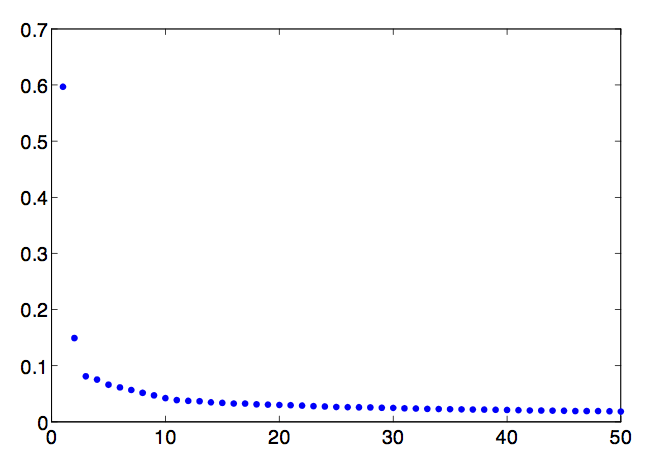
\includegraphics[scale =0.3]{../img/scree}
\end{figure}
This figure depicts the eigenvalues for an $N=1148, T = 252$ dataset of excess stock returns
\end{frame}
%%%%%%%%%%%%%%%%%%%%%%%%%%%%%%%%%%%%%%%%
\begin{frame}
	\frametitle{Choosing the Number of Factors -- Bai \& Ng (2002)}

Choose $r$ to minimize an information criterion:
$$IC(r) = \log V_r(\widehat{\Lambda}, \widehat{F}) + r \cdot g(N,T)$$
where
	$$V_r(\Lambda, F) = \frac{1}{NT}\sum_{t=1}^T (X_t - \Lambda F_t)'(X_t - \Lambda F_t)$$
and $g$ is a penalty function. The paper provides conditions on the penalty function that guarantee consistent estimation of the true number of factors. 
\end{frame}
%%%%%%%%%%%%%%%%%%%%%%%%%%%%%%%%%%%%%%%%
\begin{frame}
	\frametitle{Onatski (2013)}
	Nobody volunteered to present this paper! Unlike Bai \& Ng (2002), the idea here is \emph{not} to consistently estimate the number of factors. Instead, and in the spirit of AIC and $C_p$, we try to reconstruct the factors with minimum quadratic loss. The results in the paper apply both to ``strong'' and ``weak'' factor asymptotics.
\end{frame}

%%%%%%%%%%%%%%%%%%%%%%%%%%%%%%%%%%%%%%%%
\begin{frame}
\frametitle{What Can We Do with Factors?}

Among other possibilities:
\begin{enumerate}
	\item Use them as Instrumental Variables 
	\item Use them to construct Forecasts
	\item Use them to ``Augment'' a VAR
\end{enumerate}

\end{frame}

%%%%%%%%%%%%%%%%%%%%%%%%%%%%%%%%%%%%%%%%
\begin{frame}[c]\frametitle{Factors as Instruments -- Bai \& Ng (2010)}
\begin{block}
   	{Endogenous Regressors $x_t$}
$$y_t = x_t' \beta + \epsilon_t \quad \quad E[x_t\epsilon_t] \neq 0 $$
\end{block}   

 \begin{block}
 	{Unobserved Variables $F_t$ are Strong IVs}
$$\underset{(k\times 1)}{x_t} = \Psi'\underset{(r\times 1)}{F_t} + u_t \quad \quad E[F_t \epsilon_t] = 0$$
 \end{block}

\begin{block}
	{Observe Large Panel $(z_{1t}, \hdots, z_{Nt})$}
		$$z_{it} = \lambda_i' F_t + e_{it}$$
\end{block}

\end{frame}

%%%%%%%%%%%%%%%%%%%%%%%%%%%%%%%%%%%%%%%%

\begin{frame}[c]\frametitle{Factors as Instruments -- Bai \& Ng (2010)}

\small

$$\boxed{
	y_t = x_t' \beta + \epsilon_t, \quad \quad
	x_t = \Psi'F_t + u_t, \quad \quad
	z_{it} = \lambda_i' F_t + e_{it}
}$$
\vspace{1em}

\begin{block}
	{Procedure}
	\begin{enumerate}
		\item Calculate the PCs of Z
		\item Calculate $\widetilde{F}_t$ using the first $r$ PCs of Z
		\item Use $\widetilde{F}_t$ in place of $F_t$ for IV estimation
	\end{enumerate}
\end{block}

\begin{block}
	{Main Result}
	Under certain assumptions, as $(N,T) \rightarrow \infty$ ``estimation and inference can proceed as though $F_t$ were known.'' The resulting estimator is consistent and asymptotically normal.
\end{block}

\normalsize

\end{frame}
%%%%%%%%%%%%%%%%%%%%%%%%%%%%%%%%%%%%%%%%
\begin{frame}[c]\frametitle{Factors as Instruments -- Bai \& Ng (2010)}
    
\begin{block}
	{Why Might This be Helpful?}
	\begin{enumerate}
		\item Avoid many instruments bias
		\item Avoid bias from irrelevant instruments
		\item Allow more observed instruments $z_{it}$ than sample size $T$
		\item Provided that $\sqrt{T}/N \rightarrow 0$, all of the observed instruments $z_{it}$ can be \emph{endogenous} as long as $F_t$ is exogenous
	\end{enumerate}
\end{block}

\end{frame}
%%%%%%%%%%%%%%%%%%%%%%%%%%%%%%%%%%%%%%%%
\begin{frame}[c]\frametitle{Forecasting with Dynamic Factors}
    
 \begin{itemize}
 	\item Similar to Principal Components Regression (PCR)
 	\item Estimate factors $\widehat{F}_t$ from a large number of regressors $X_t$
 	\item Run a regression to forecast $y_t$ using $\widehat{F}_t$ rather than $X_t$ 
 \end{itemize}

\vspace{2em}

\alert{We'll talk about this more next time and compare to other high-dimensional forecasting procedures.}

\end{frame}
%%%%%%%%%%%%%%%%%%%%%%%%%%%%%%%%%%%%%%%%
\begin{frame}[c]\frametitle{FAVARs -- Bernanke, Boivin \& Eliasz (2005)}
   
   \begin{block}
    	{Two Problems with Structural VARs}
    	\begin{enumerate}
    		\item Number of parameters is \emph{quadratic} in the number of variables. Unrestricted VAR infeasible unless $T$ is large relative to $N$.\begin{itemize}
    			\item You've studied one solution to this problem already this semester: Bayesian Estimation with informative priors 
    		\end{itemize}
    		\item To keep estimation tractable we typically use a small number of variables, but then the VAR innovations ``might not span the space of structural shocks.''
    	\end{enumerate}
    \end{block} 


\end{frame}

%%%%%%%%%%%%%%%%%%%%%%%%%%%%%%%%%%%%%%%%
\begin{frame}[c]\frametitle{FAVARs -- Bernanke, Boivin \& Eliasz (2005)}

\begin{block}{Factor-Augmented VAR Model}
	\begin{eqnarray*}
		\left[\begin{array}
			{c} Y_t \\ F_t
		\end{array} \right] &=& \Phi(L)\left[\begin{array}
			{c} F_{t-1} \\ Y_{t-1}
		\end{array} \right] + v_t\\ \\
		X_t &=& \Lambda^f F_t + \Lambda^y Y_t + e_t
	\end{eqnarray*}

\vspace{2em}

\small
$\underset{(M\times 1)}{Y_t} = $  observable variables that ``drive dynamics of the economy''\\ \vspace{1em}
$\underset{(K\times 1)}{F_t} = $ Small \# of unobserved factors: ``additional information''\\ \vspace{1em}
$\underset{(N\times 1)}{X_t} = $ Large \# of observed ``informational time series''
\end{block}

\end{frame}
%%%%%%%%%%%%%%%%%%%%%%%%%%%%%%%%%%%%%%%%
\begin{frame}[c]\frametitle{FAVARs -- Bernanke, Boivin \& Eliasz (2005)}

\small
$$\boxed{\quad \left[\begin{array}
			{c} Y_t \\ F_t
		\end{array} \right] = \Phi(L)\left[\begin{array}
			{c} F_{t-1} \\ Y_{t-1}
		\end{array} \right] + v_t \quad \quad \quad \quad
		 X_t = \Lambda^f F_t + \Lambda^y Y_t + e_t \quad}$$
\normalsize

\begin{block}{Consider Two Estimation Procedures}
	\begin{enumerate}
		\item Two-step Procedure:\begin{itemize}
			\item Estimate space spanned by factors using first $K + M$ PCs of $X$
			\item Estimate VAR with $\widehat{F}_t$ in place of $F_t$
		\end{itemize}
		\item Full Bayes (Gibbs Sampler)
	\end{enumerate}
\end{block}

\begin{block}{Empirical Application}
Additional information contained in FVAR is ``important to properly identify the monetary transmission mechanism.''
\end{block}
\end{frame}
%%%%%%%%%%%%%%%%%%%%%%%%%%%%%%%%%%%%%%%%
\end{document}
